\chapter{Extension of the Rule-Based Lloyd Algorithm to 3D\label{chap:rbl}}

\section{Introduction to the RBL}

This chapter will contain overview of the RBL algo in 2d, with some key principles for motion planning, safety and convergece. Also some applications and limitations in 2d. TODO del

    \subsection{Overview}

        RBL, as presented in the original paper \cite{rbl_paper}, ensures convergence to the goal and provides sufficient conditions for achieving it. 
        The problem involves individual control of $N$ agents from their initial position $\mathbf{p}_i(0)$ toward a goal region, represented as circle.
        This goal region is denoted as $B(\mathbf{e}_i, \epsilon)$, where $\mathbf{e}_i$ is center and $\epsilon$ is radius of goal region.
        Each agent is knows of its current position $\mathbf{p}_i$, encumbrance $\delta_i$, which determines safe space around agent.
        Additionally, each agent also knows the positions and encumbrances of its neighboring agents $\mathbf{\mathcal{N}_i}$, agent $j \in \mathbf{\mathcal{N}_i}$ if $||\mathbf{p}_i - \mathbf{p}_j|| \leq 2r_{s,i}$, where $r_{s,i}$ is denoted as half of the sensing radius of the i-th agent.
        For simplicity $r_{s,i}$ is considered to be same for all agents, therefore $r_{s,i} = r_s$. 

        TODO, write limitations and motivation for extension here.

    \subsection{Key principles}

        The core idea is to minimize the following cost funciton: 
        \begin{equation}
            J_{cov}(\mathbf{p}) = \sum_{i=1}^{N} \int_{\mathcal{V}_i} \lVert\mathbf{q}-\mathbf{p}_i\rVert^2 \phi_i (\mathbf{q})d\mathbf{q},
            \label{coverage_cost_function}
        \end{equation}
        where $\mathbf{p}_i$ is the position of agent $i$, $\mathcal{V}_i$ is the Voronoi cell of the i-th robot, $\lVert\mathbf{q}-\mathbf{p_i}\rVert^2$ is squared Euclidian distance between point in the mission space $\mathbf{q} \in \mathcal{Q}$ and agent's position $p_i$, 
        and $\phi_i (\mathbf{q})$ is the weighting function.

        Voronoi cell is defined as: 
        \begin{equation}
            \mathcal{V}_i = \{q \in \mathcal{Q} \lvert \lVert \mathbf{q} - \mathbf{p}_i \rVert \leq \lVert q - \mathbf{p}_j \rVert, \forall j \neq i\}
        \end{equation},
        for visual representation see \reffig{fig:voronoi_2d}. 
        However, this standard definition of Voronoi cells does not take into account the physical space occupied by the agents, or their encumbrances. 
        To address this, a Modified Voronoi cell is introduced, which takes into account the encumbrances of agents.
        This modified version adjusts the boundaries of each Voronoi cell to account for the encumbrances of neighboring agents.
        The modified Voronoi cell definition is as follows:
        \begin{equation}
            \tilde{V}_i = 
            \begin{cases}
            \{ \mathbf{q} \in Q \mid \| \mathbf{q} - \mathbf{p}_i \| \leq \| \mathbf{q} - \mathbf{p}_j \| \}, & \text{if } \Delta_{ij} \leq \frac{\| \mathbf{p}_i - \mathbf{p}_j \|}{2} \\
            \{ \mathbf{q} \in Q \mid \| \mathbf{q} - \mathbf{p}_i \| \leq \| \mathbf{q} - \tilde{\mathbf{p}}_j \| \}, & \text{otherwise},
            \end{cases}
        \end{equation}
        $\forall j \in \mathcal{N}_i$, where $\Delta_{ij} = \delta_i + \delta_j$ and $\tilde{\mathbf{p}}_j = \mathbf{p}_j + 2(\Delta_{ij} - \frac{\| \mathbf{p}_i - \mathbf{p}_j \|}{2})\frac{ \mathbf{p}_i - \mathbf{p}_j }{\| \mathbf{p}_i - \mathbf{p}_j \|}$.

        \begin{figure}[H]
            \centering
            \subfloat[Euclidean Voronoi Diagram in 2D] {
            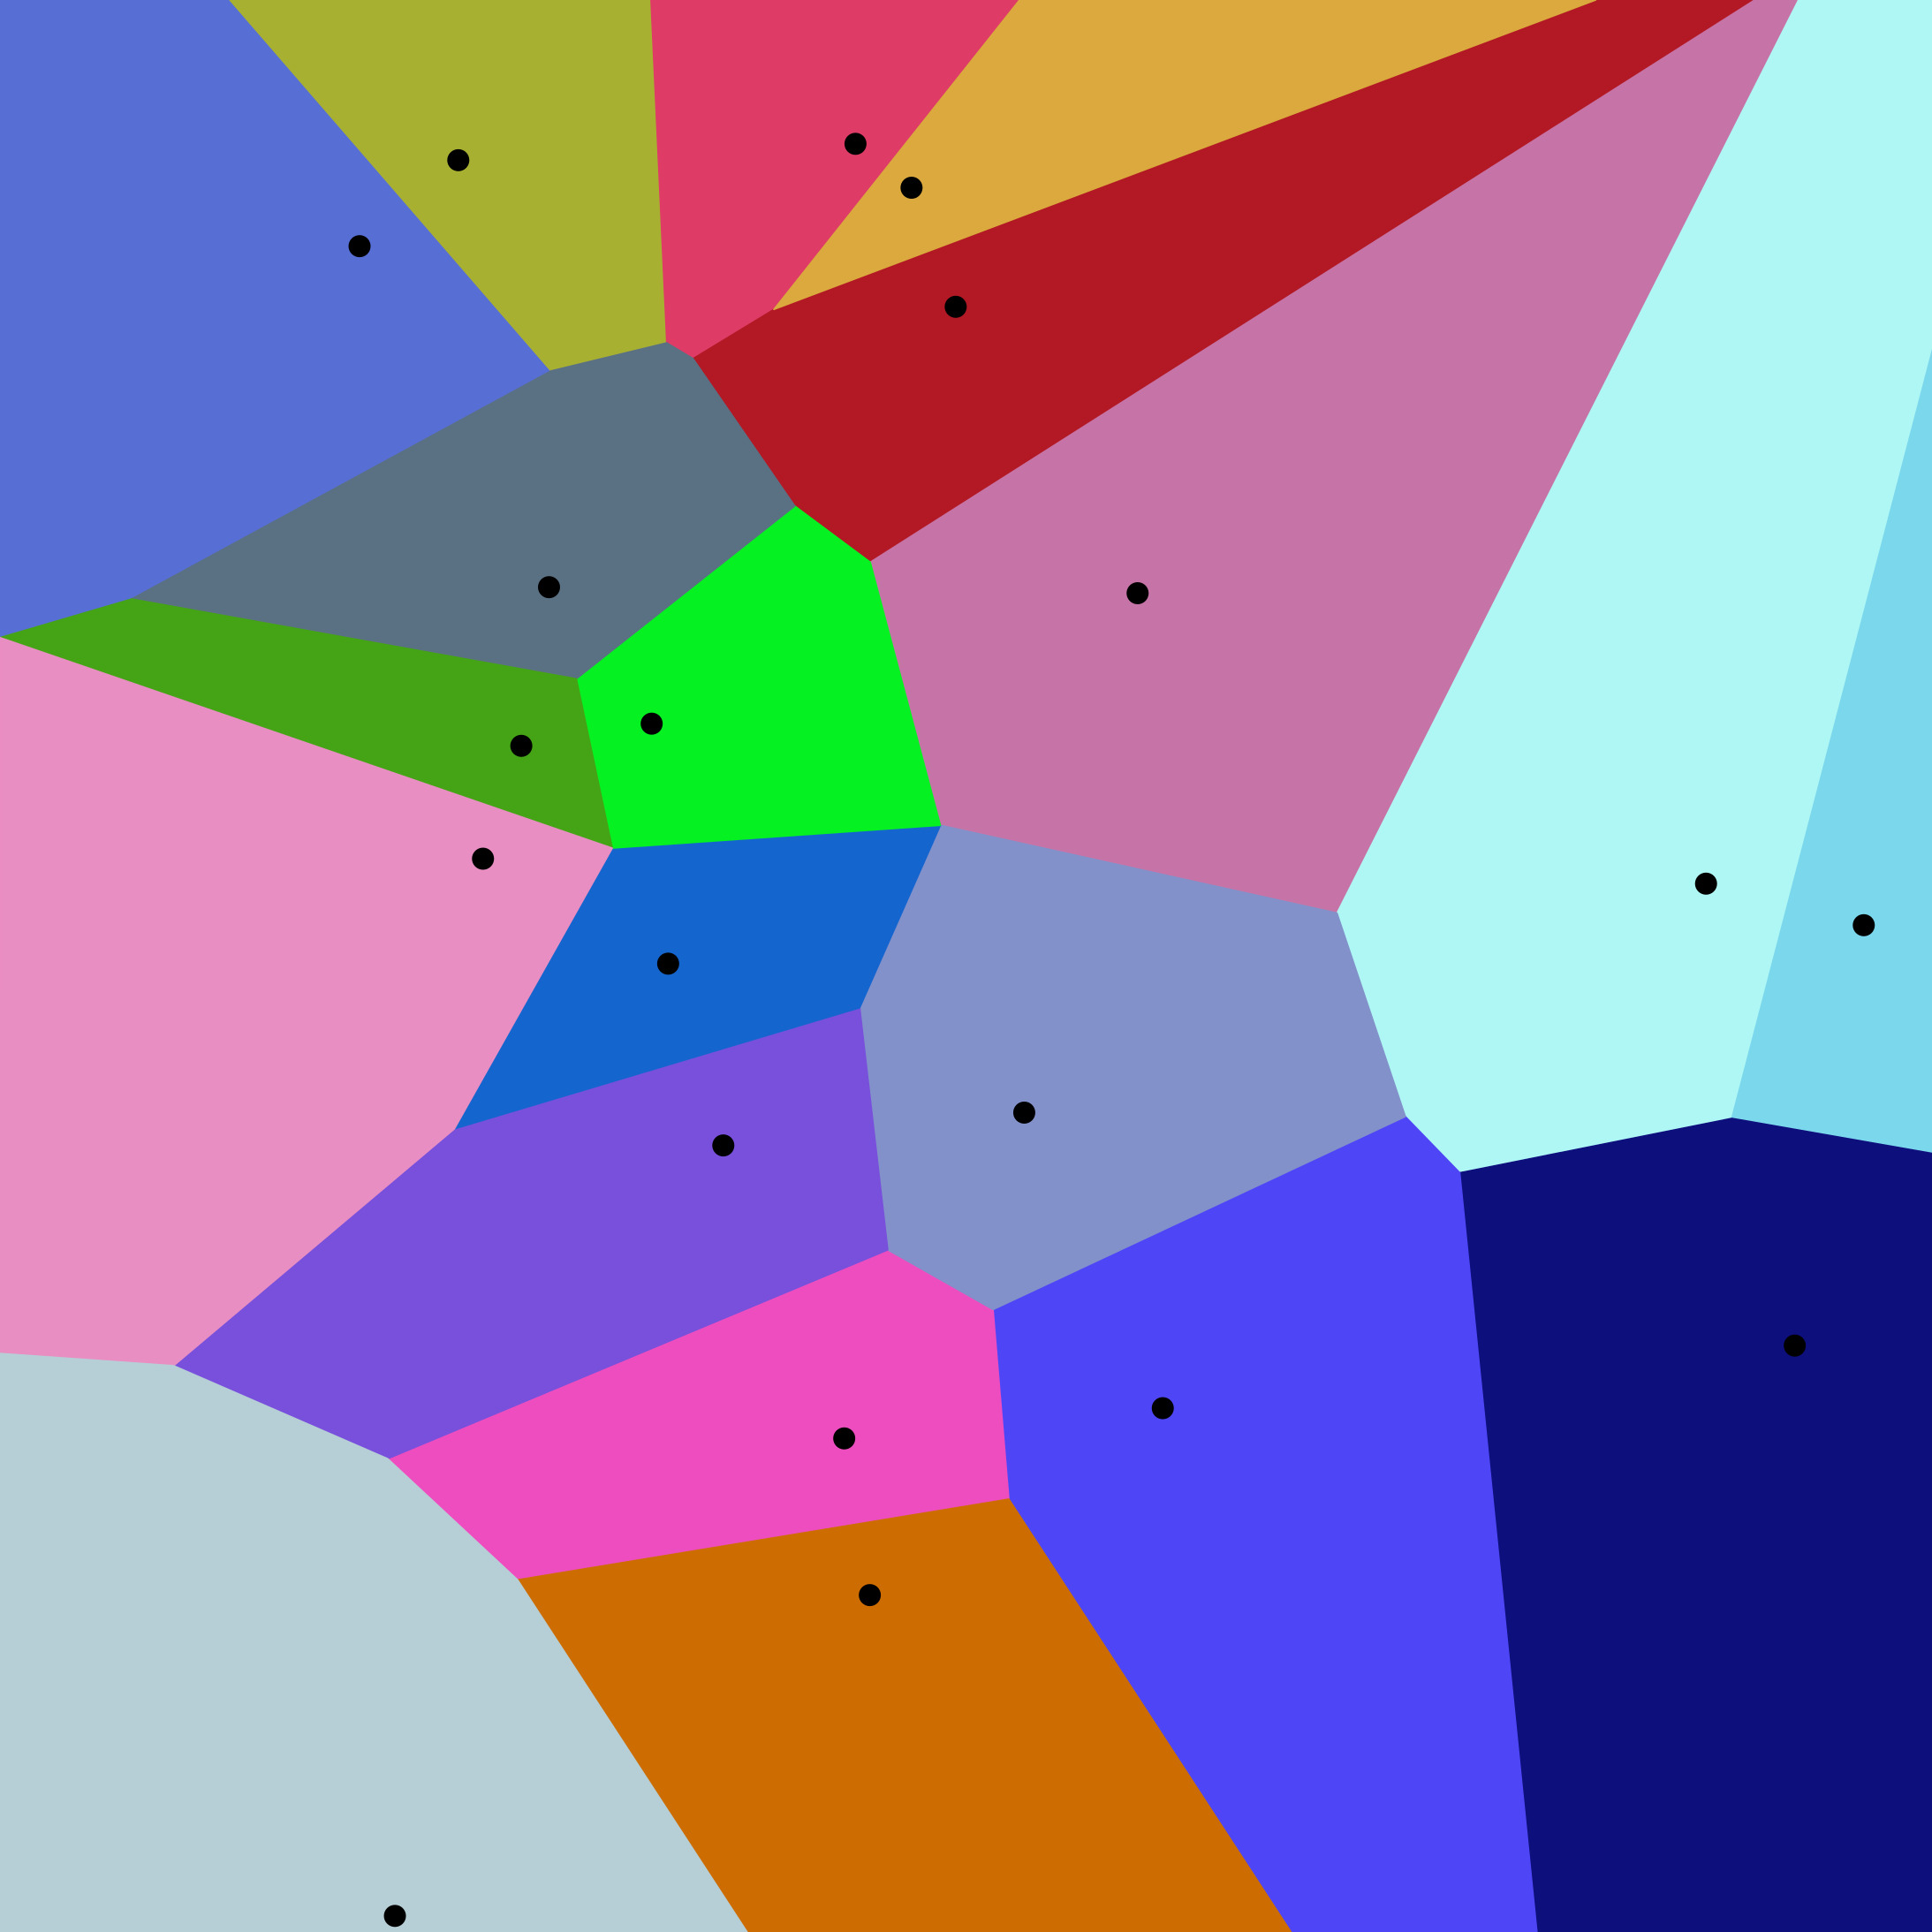
\includegraphics[width=0.48\textwidth, height=0.48\textwidth]{./fig/diagrams/Euclidean_Voronoi_diagram.jpg}
            \label{fig:voronoi_2d}
            }
            \subfloat[Euclidean Voronoi Diagram in 3D] {
            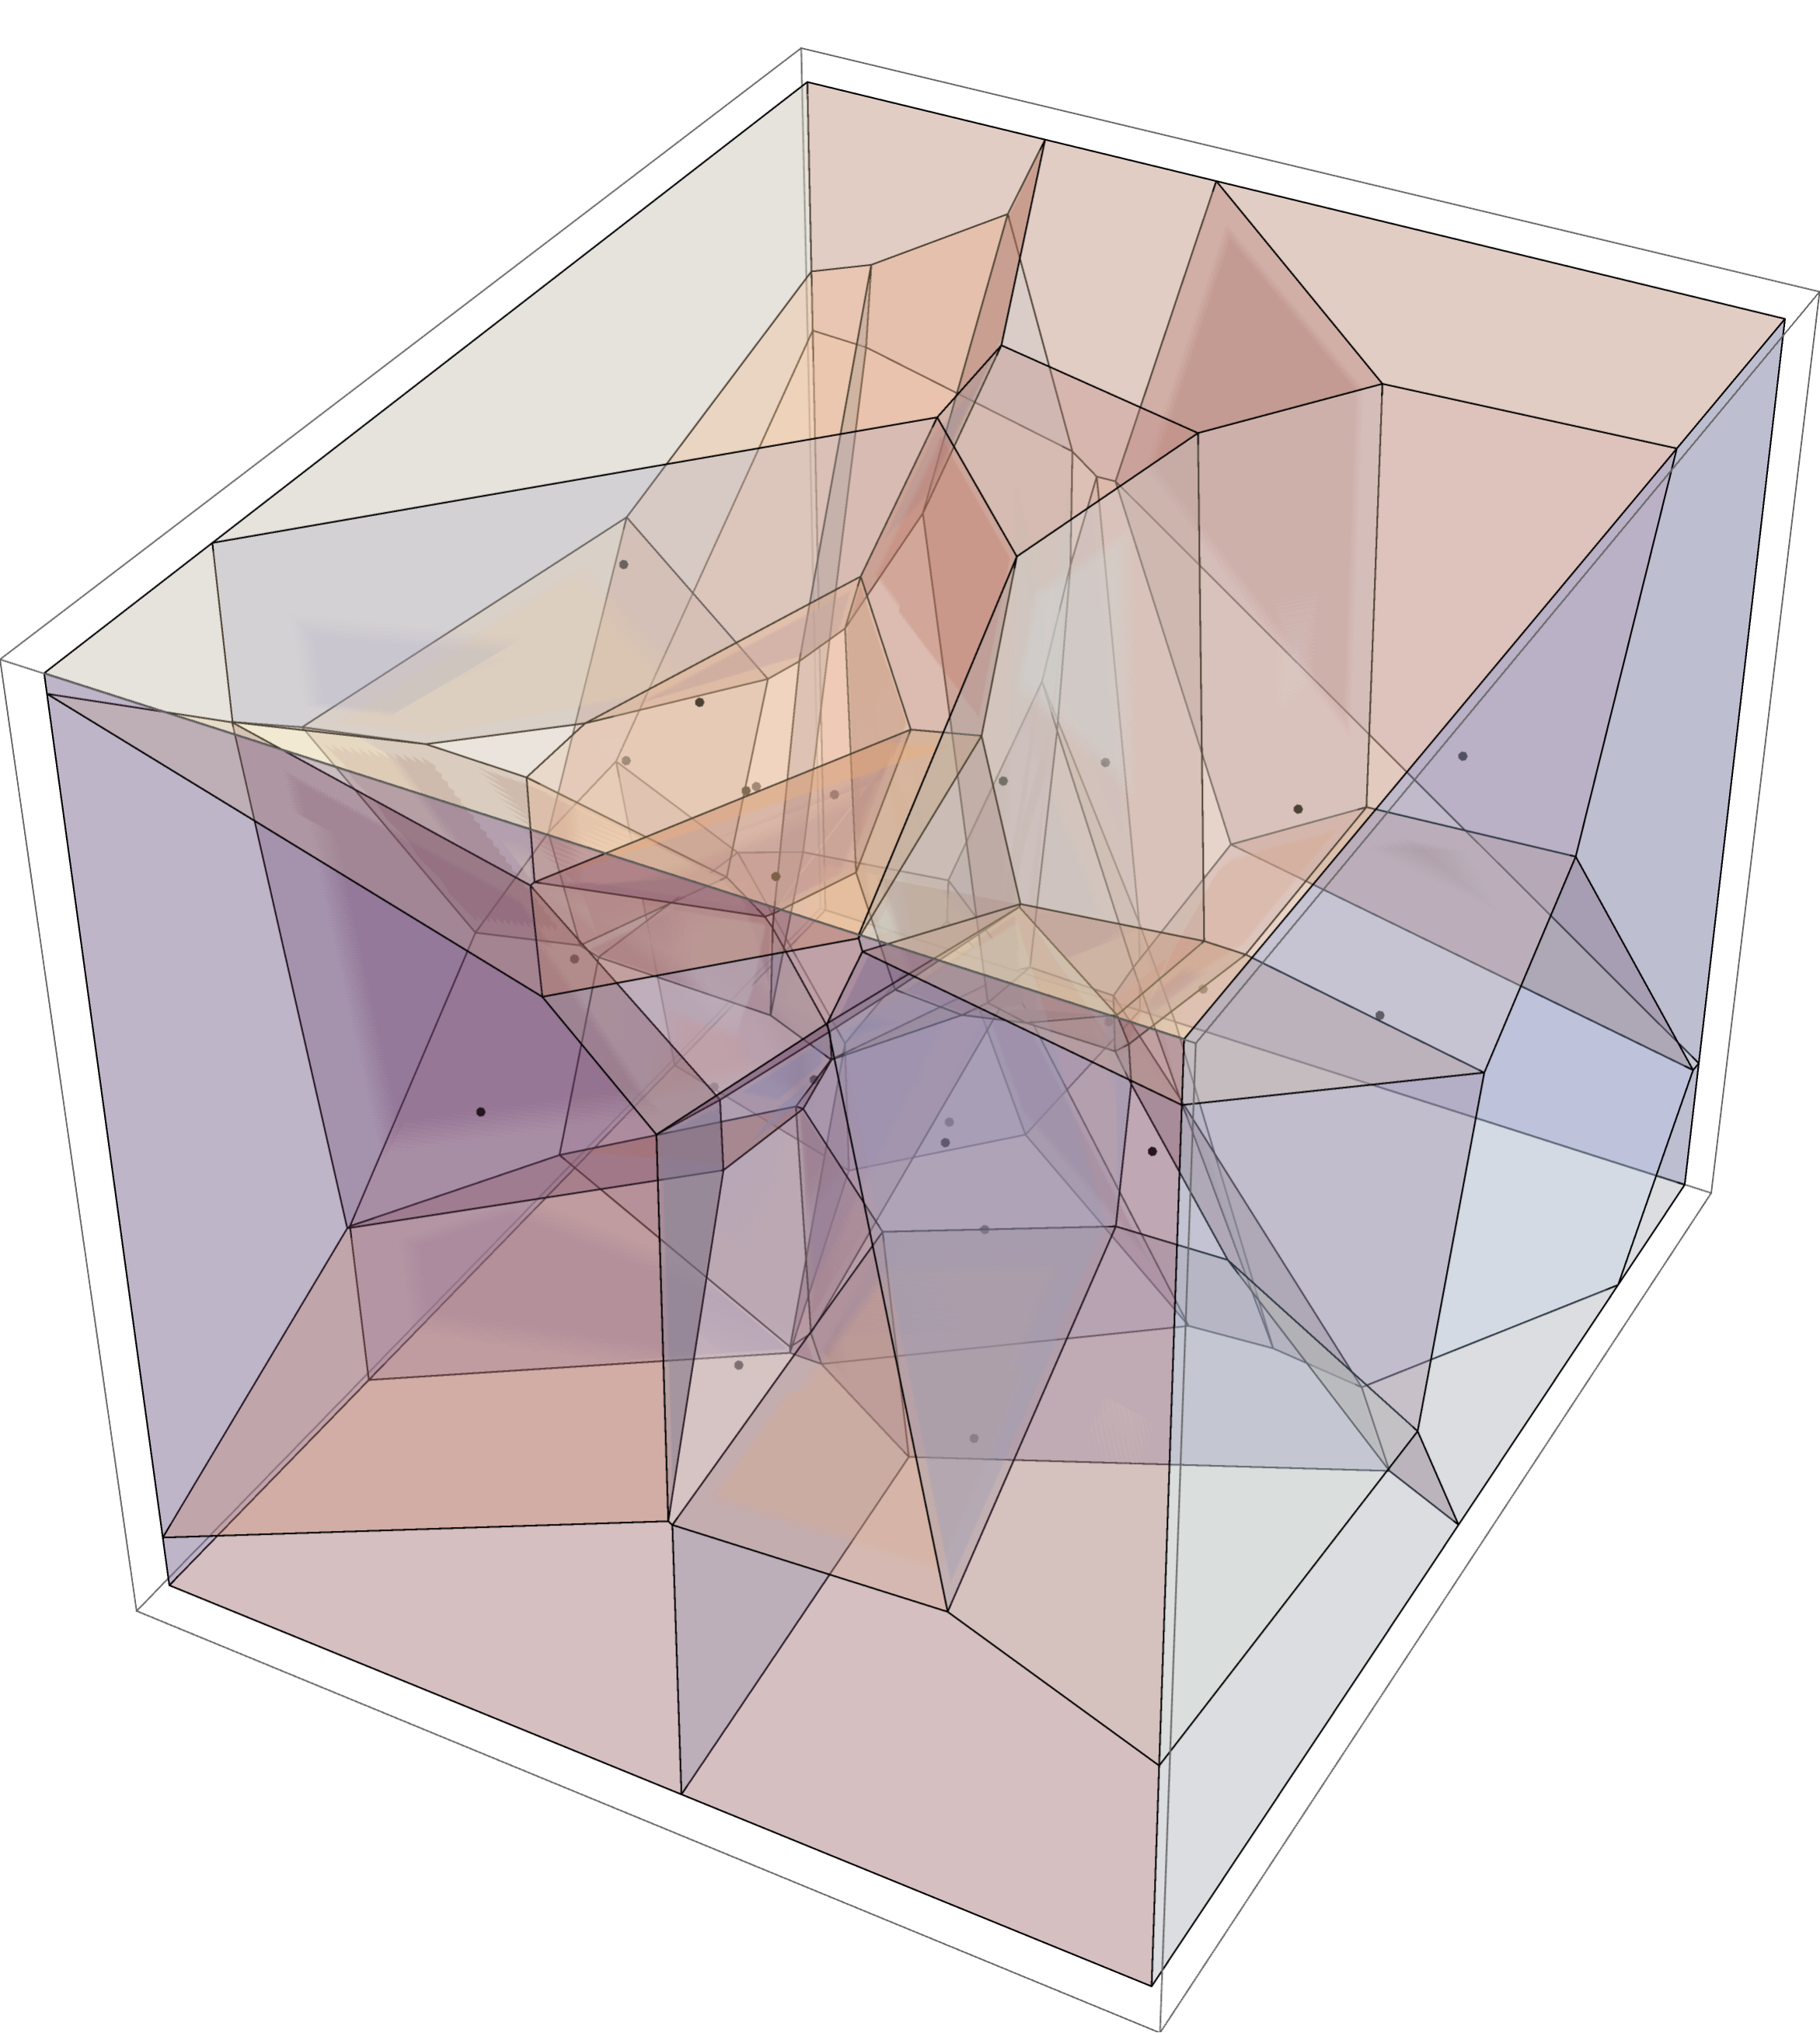
\includegraphics[width=0.48\textwidth, height=0.48\textwidth]{./fig/diagrams/Euclidian Voronoi diagram 3d.png}
            \label{fig:voronoi_3d}
            }
            \caption{
                (a) an example of 20 Voronoi cells in 2D \cite{Voronoi2d} (b) 25 Voronoi cells in 3D \cite{Voronoi3d}
            }
            \label{fig:voronoi_diagrams}
        \end{figure}

        Convergence to goal reagion $B(\mathbf{e}_i, \epsilon)$ depends on the choice of weighting function that assigns weights to points $\mathbf{q}$ in the mission space $\mathcal{Q}$.
        The weighting function $\phi_i(\mathbf{q})$ is defined as follows: 

        \begin{equation}
            \phi_i(\mathbf{q}) = \exp\left(-\frac{\|\mathbf{q} - \bar{p}_i\|}{\beta_i}\right) \tag{7}
        \end{equation}
        
        where
        
        \begin{equation}
            \dot{\beta}_i(A_i) = 
            \begin{cases}
                -\beta_i & \text{if } \|\mathbf{c}_{A_i} - \mathbf{p}_i\| < d_1 \land \|\mathbf{c}_{A_i} - \mathbf{c}_{S_i}\| > d_2, \\
                -(\beta_i - \beta_i^D) & \text{otherwise.}
            \end{cases} \tag{8}
        \end{equation}
        
        \begin{equation}
            \dot{\bar{p}}_i = 
            \begin{cases}
                -(\bar{p}_i - R\mathbf{p}_i (\frac{\pi}{2} - \epsilon) \mathbf{e}_i) & \text{if } \|\mathbf{c}_{A_i} - \mathbf{p}_i\| < d_3 \land \|\mathbf{c}_{A_i} - \mathbf{c}_{S_i}\| > d_4, \\
                -(\bar{p}_i - \mathbf{e}_i) & \text{otherwise,}
            \end{cases}
        \end{equation}
        
        where 
        
        \[
        \bar{p}_i = 
        \begin{cases}
        \mathbf{e}_i & \text{if } \|\mathbf{p}_i - \mathbf{c}_{A_i}\| > \|\mathbf{p}_i - \mathbf{c}_{A_i}\|, \\
        R\mathbf{p}_i (\frac{\pi}{2} - \epsilon) \mathbf{e}_i & \text{otherwise.}
        \end{cases}
        \]
            

        
        The position of the centroid \( \mathbf{c}_{V_i} \) of a region \( V_i \), weighted by the function \( \phi_i(q) \), is used to guide the control. It is defined as:

        \begin{equation}
            \mathbf{c}_{V_i} = \frac{\int_{V_i} \mathbf{q} \phi_i(\mathbf{q}) \, d\mathbf{q}}{\int_{V_i} \phi_i(\mathbf{q}) \, d\mathbf{q}},
        \end{equation}

        where \( \mathbf{q} \) represents the position vector, and \( \phi_i(\mathbf{q}) \) is a weighting function. The centroid \( \mathbf{c}_{V_i} \) serves as the target for the control system, directing the system toward the weighted center of the region.




    \subsection{Applications in 2D}

    \subsection{Limitations in 2D}


\section{Motivation for 3d Extension}

Importance and challenges

\section{Mathematical Describtion in 3D}

modified voronoi partitioning, transition from planar 2d to spatial 3d, safety and convergence in 3d.

\section{Simulation and Results Analysis}

Describtion of simulation enviroment, used tools, Describtion of few simulation scenarios and result analysis.

\section{Summary and Key Insights}

Recap of modifications. Faced challenges and solutions applied
